%!TEX root = ../report.tex

\begin{document}
  \chapter{Experimental Setup}

  Having applied the theoretical knowledge derived in Section 3 to the ROPOD case
  study in Section 4 we have begun to narrow down the options for spatio-temporal
  world modeling in this particular case. However, a theoretical comparison will
  only suffice for so long. Given the focus ROPOD places on real world
  environments it is critical that some operational tests be preformed before
  method selection. Not only will these experiments serve as a guide for ROPOD,
  but they will also act as a template for the comparison of future
  spatio-temporal world modeling techniques.


  \section{ Environmental Representation}

  Given the complexity and size of the target environment for ROPOD, a large
  hospital, it is necessary to pair down features of the building until only the
  core components remain. The three dynamic environmental components being
  target are doors, elevators, and carts that are often strewn about the
  hallways and surrounding rooms. Therefore, a model environment has been
  designed for the simulations to be run on that contains these three key
  components.  The model environment that has been designed takes heavy
  influence from the actual environment but some notable have been made. The
  model has a decreased area to allow for faster model training and path
  planning. Additionally, extraneous rooms and hallways have been removed. A
  comparison between the actual hospital and the designed model can be seen below.

  TODO add picture


  \section{ Common Assumptions }
  In order to insure only the desired component is being tested at any given
  time a set of assumptions are made.

  \begin{itemize}

    \item All robot components are working correctly (no internal faults)

    \item Other than the object under test (e.g. doors), all other objects in the
          environment are static

    \item All information other than the objects under test are perfectly known

    \item Observations made/provided by the training data are assumed to be ground-truth

  \end{itemize}


  \section{ Commonalities in Approach }
  Although different components will be under test, each experiment will be run
  in a similar manor.

  The experimental setup is as follows:

  \begin{itemize}

    \item Training data consisting of observations made every 10 minutes over a simulated month will
          be provided to the models

    \item 3 training sets will be made:
      \begin{itemize}

        \item TODO further discuss generation of datasets

        \item Highly consistent generation

        \item Generation consistent with early periodicity of data obtained

        \item Data with higher chance of abnormalities

      \end{itemize}

    \item Using the same generation procedure, a set of three new months will be
          generated

    \item 4 times will be randomly selected each day of the month using a
          uniform distribution for which the models must generate maps

    \item An optimal path using the ground truth will be generated for each of
          these time slots using the selected models

    \item Additionally, maps will be generated using the ground truth, best
          case, and worst case, assumptions

    \item All of these paths will then be compared using the criteria described
          below.

    \item TODO what about a test with sparseness of data

    \item All experiments will be done on the same hardware
      \begin{itemize}
        \item Desktop PC
        \item i7-2600k 3.4GHz
        \item 8GB DDR3
        \item Ubuntu 14.04 Trusty Tahr
      \end{itemize}

  \end{itemize}


  \section{ Comparison Criteria }
  In order to evaluate the intricacies of the selected models a wide variety of
  data points have been selected for comparison. A focus has been placed on collecting
  data relevant to scale-ability of the modeling technique given the eventual scope of the ROPOD project.

  \begin{itemize}

    \item Accuracy to Ground Truth

    \item Accuracy to Historical Recreations

    \item Planning Run-time

    \item Planning Memory Consumption

  \end{itemize}


  \section{ Doored Areas}

  \subsection{ Experimental Motivation }

  As is the case in many places of employment many areas of a building may not
  be accessible to the public, and by extension the robots, outside of work
  hours.  This could come in the form of a given hallway between two areas being
  locked after 17:00 as the day works go home. In another case, it could be as
  simple as someone preferring to having a door shut to a hallway during a loud
  or chaotic time of the day. \\

  Regardless of the reason, it is certain that the states of doors are often
  both dynamic and periodic. In the ideal case, a robot, much like humans,
  would learn when certain doors are closed and be able to plan accordingly.
  Making an accurate prediction can save time, but making an inaccurate
  predication can also be costly. An in accurate prediction would force a robot
  to not only backtrack, but also recalculate that path required to get to a
  target. Additionally, it may not be possible to make deliveries at all times.
  In the worse case, a robot may even manage to get itself locked in an
  environment unable to return back to it's base and eventually run out of power
  requiring human intervention. For these reasons and many more, the door
  experiment is an excellent example of the benefits of spatio-temporal world
  modeling. \\

  \subsection{ Experimental Details }

  In order to keep this test as straight forward as possible, only one door has
  been included. The door belongs to a room that where a package must be
  delivered Each model will be directly, or indirectly be tasked with predicting
  the state of this door. Figure 5.1 displays the starting and goal point of
  the desired path. A simple 50\% confidence value will be used. That is to
  say, if a model predicts that the door will be 50\% or more likely to be open
  will result in the robot attempting to deliver the package.


  \begin{figure}[!htb]
    \centering
    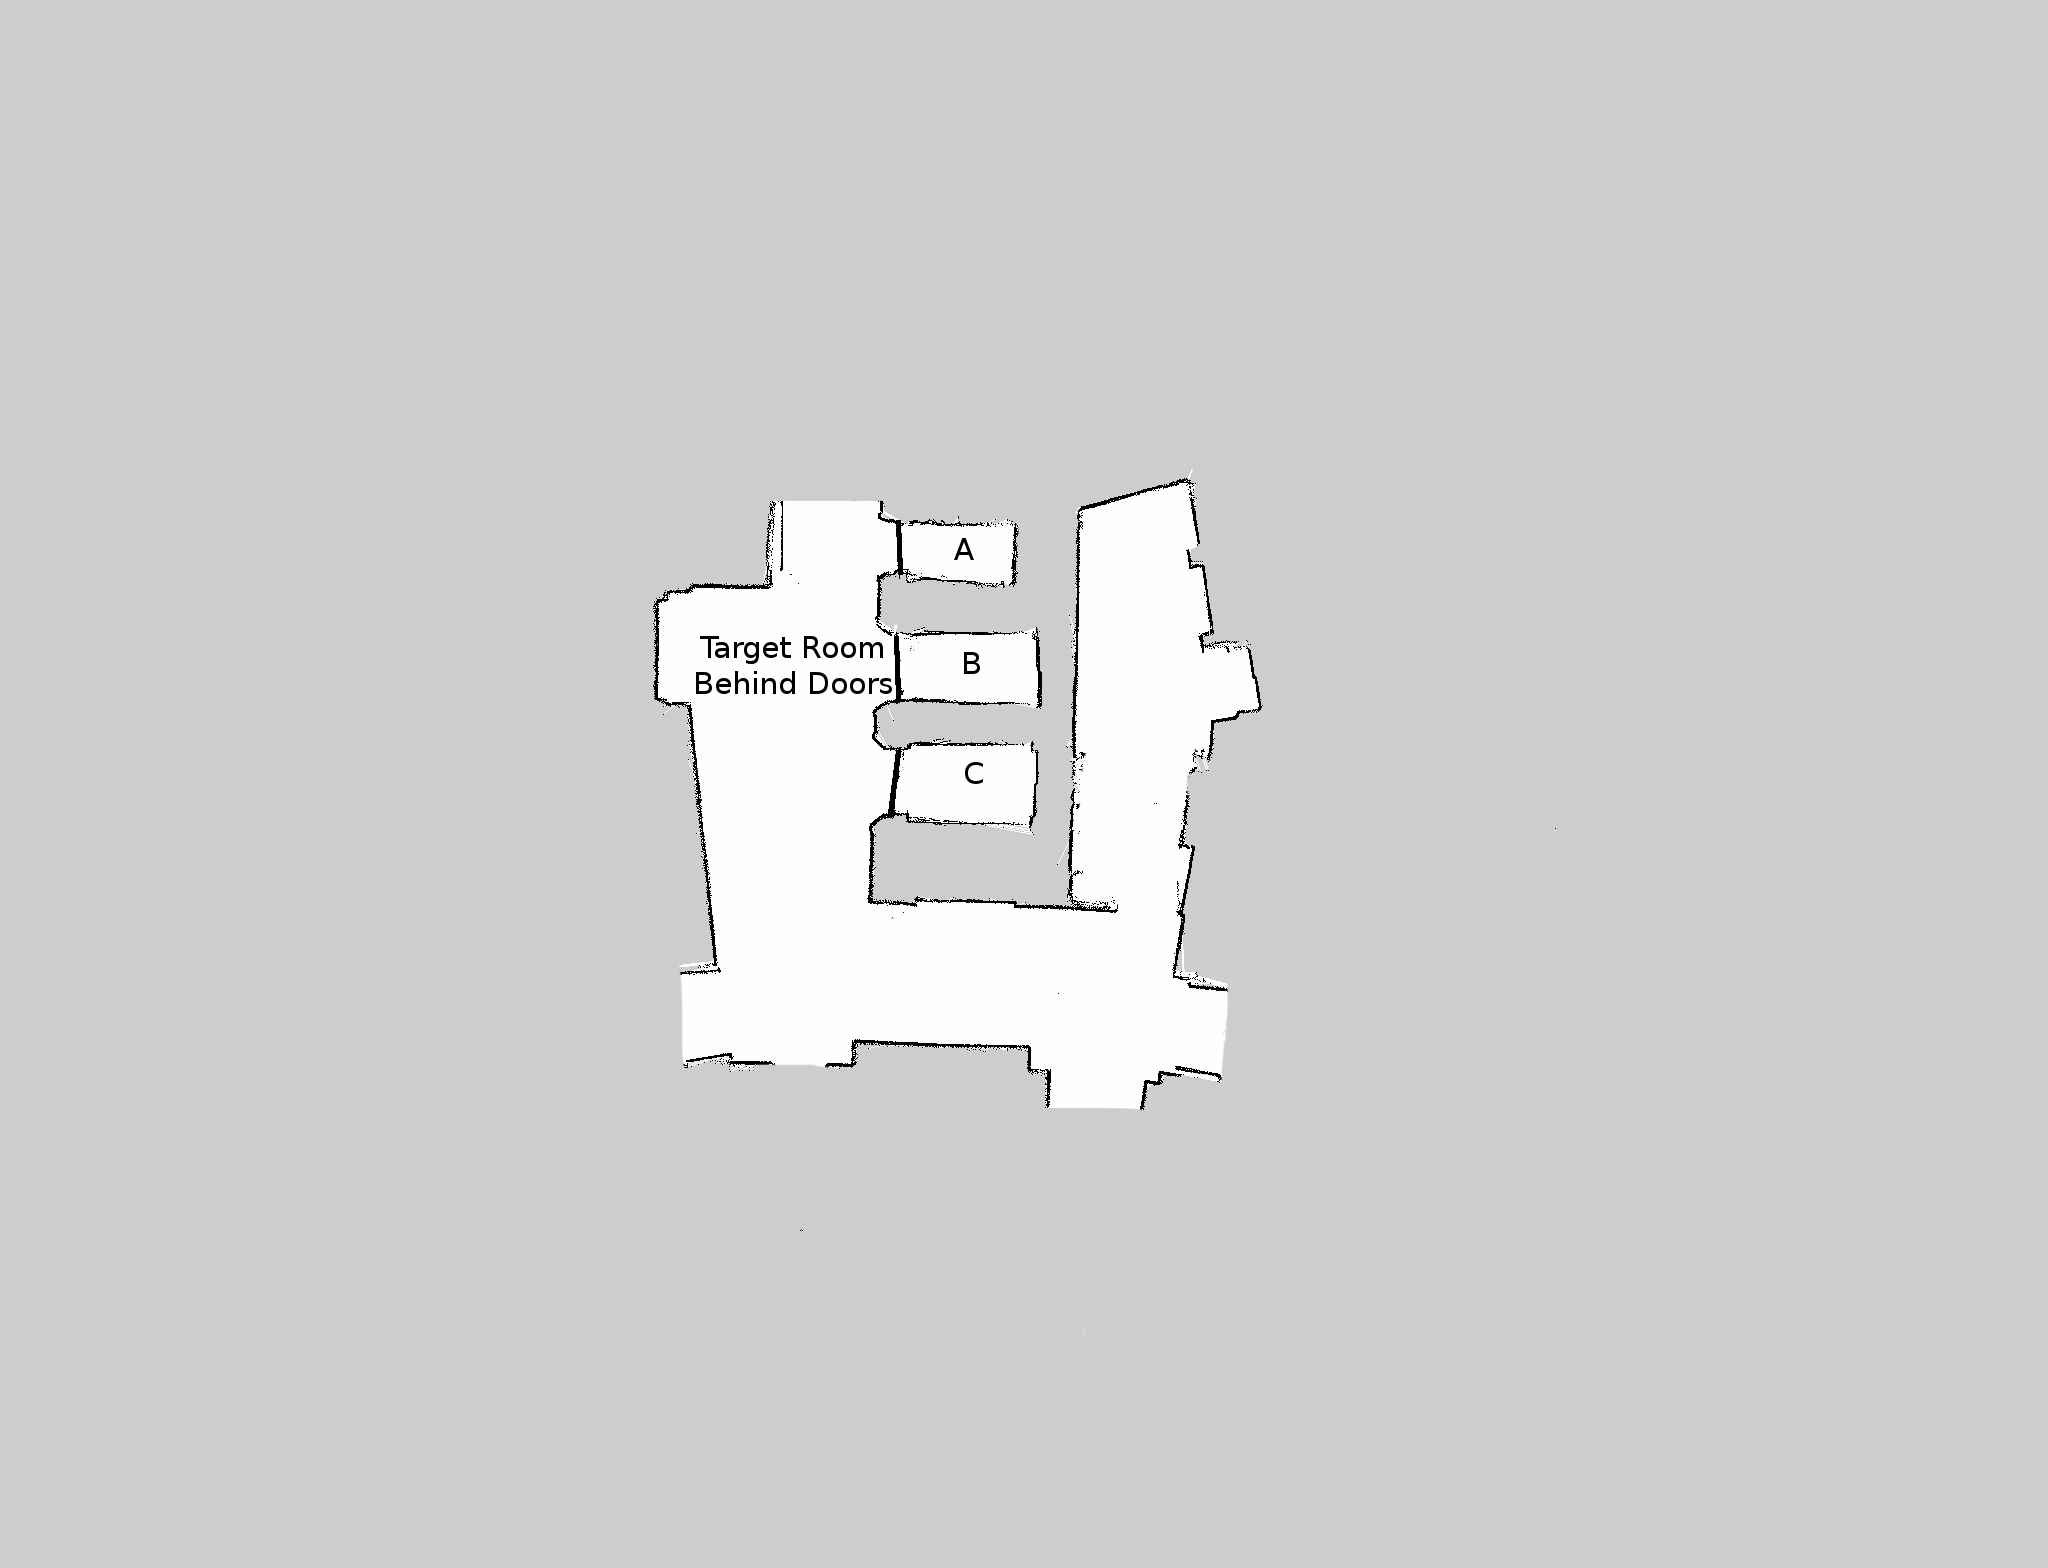
\includegraphics[width=\linewidth]{images/ward_24_door.png}
    \caption{Multiple rooms behind doors in ward 24.}
    \label{figure:ward_24_door}
  \end{figure}

  TODO should I include something like this here or elsewhere?
  It is clear that this 50\% cutoff does not take into account the penalties of
  making a wrong prediction, but this experiment was designed to investigate the
  accuracy of the prediction. How the information of the prediction is handled
  afterwards is undoubtedly valuable, but is outside the scope of this current
  research.

  \
  TODO include description of how the simulation was generated.


  \section{ Congested Hallways }

  \subsection{ Experimental Motivation }



  \subsection{ Experimental Details }

  Figure 5.3 displays the starting and goal point of the
  desired path. In order to keep this test as straight forward as possible, only
  one door has been included. The door belongs to a hallway that acts like a
  shortcut between the two other hallways. Each model will be directly, or
  indirectly tasked with predicting the state of this door. A simple 50\%
  confidence value will be used. That is to say, if a model predicts that the
  door will be 50\% or more likely to be open that path will be taken. \\


  \begin{figure}[!htb]
    \centering
    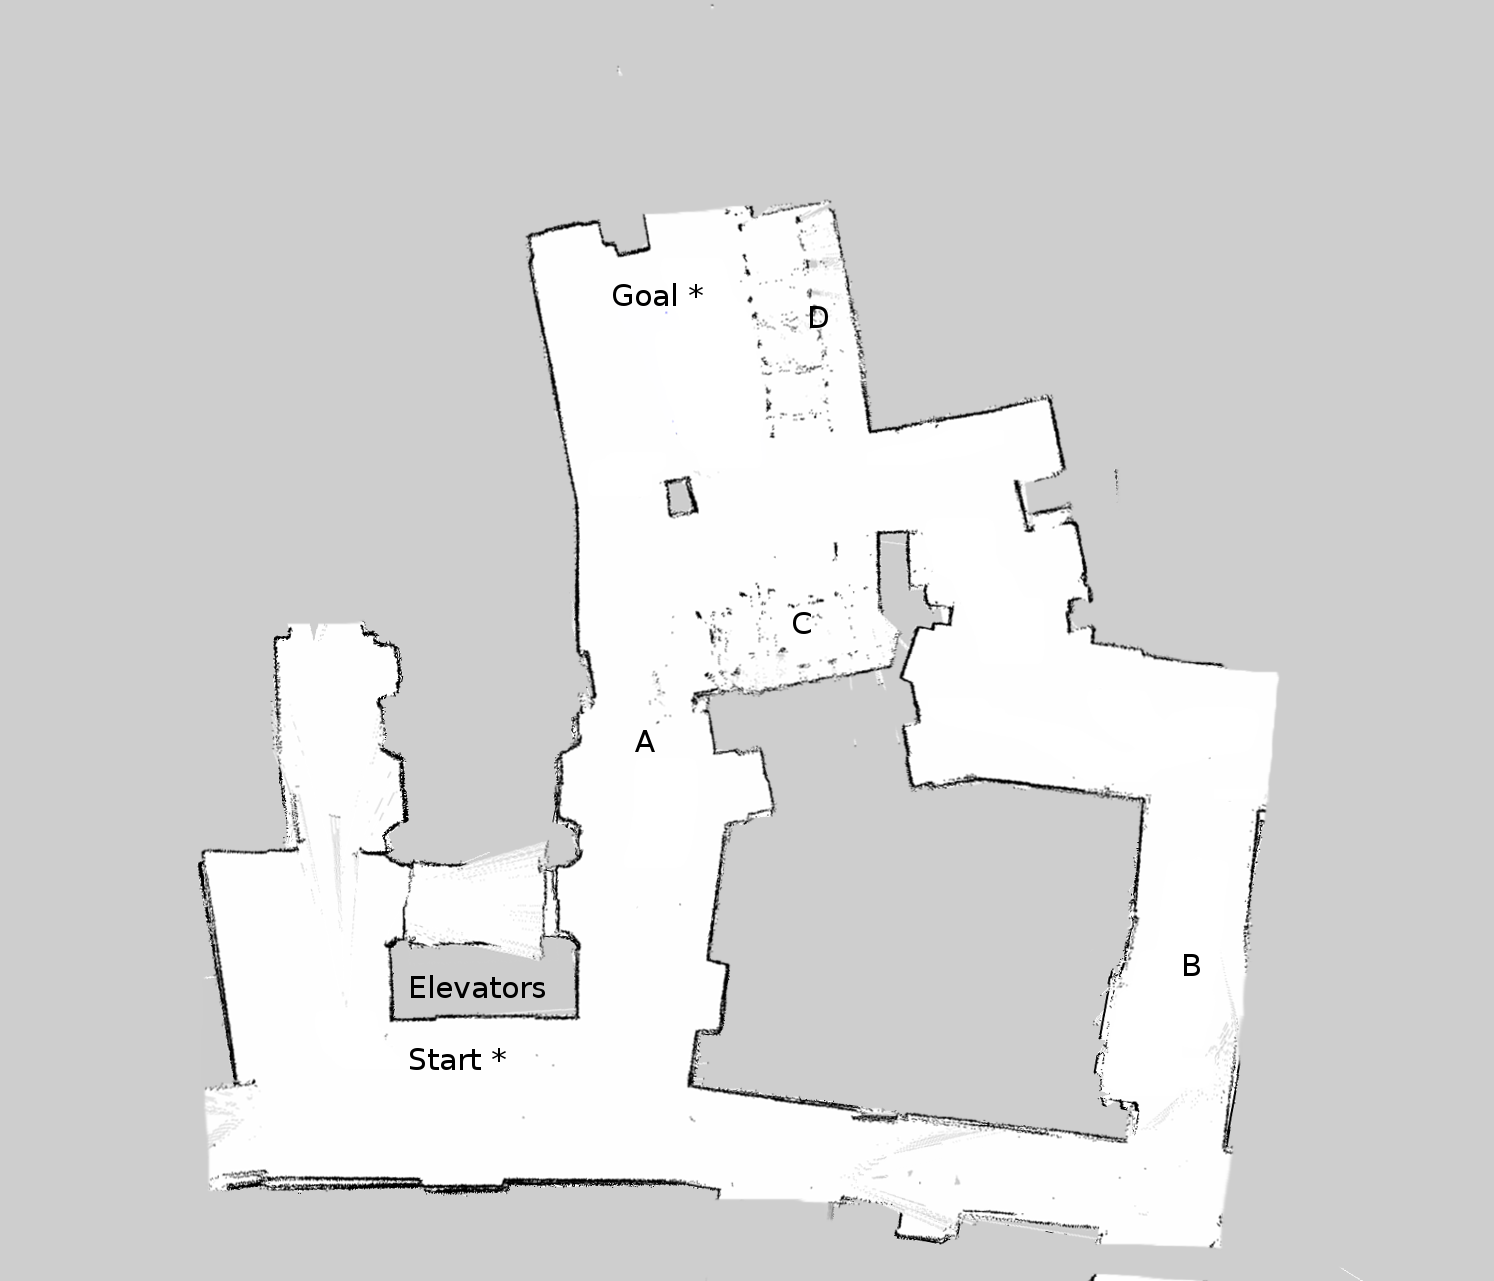
\includegraphics[width=\linewidth]{images/basement_congestion.png}
    \caption{The path from the elevator to the storage area is often congested. }
    \label{figure:basement_congestion}
  \end{figure}


  TODO include description of how the simulation was generated.
\end{document}
